\documentclass[]{beamer}
% \geometry{papersize={16cm,9.60cm}}
\usepackage{etex}
\usepackage{amsmath}
\usepackage{tikz}
\usepackage{multimedia}
\usetheme{Boadilla}
\usepackage{graphicx}
\usepackage{url}
%\usepackage{inputenc}

% \mode<presentation>
% {
%   \usetheme{default}
%   \setbeamercovered{transparent}
% }


% {\vskip5pt}

%% customize layout, bullet points navigation toolbar
\setbeamertemplate{navigation symbols}{}%remove navigation symbols
\setbeamertemplate{enumerate items}[default]
\setbeamertemplate{navigation symbols}{}
\setbeamertemplate{itemize items}[circle]
\setbeamercolor{enumerate item}{fg=black}

\setbeamertemplate{footline}{}
\setbeamersize{text margin left = 2.0em}
\setbeamersize{text margin right = 2.0em}

\usepackage{times}
\usepackage[T1]{fontenc}

% Or whatever. Note that the encoding and the font should match. If T1
% does not look nice, try deleting the line with the fontenc.

\setbeamertemplate{navigation symbols}{}

\title{ Cognitive (Neuro) Psychology }
\subtitle{V. Perceiving and recognizing objects}
\author{ Marianne Maertens }
\institute[TU Berlin]{Technische Universit\"at Berlin}
\date{July 2016}

\begin{document}
\setbeamertemplate{enumerate items}[default]
\setbeamertemplate{headline}

\frame{\titlepage}

\AtBeginSection[]
{
  \begin{frame}<beamer>
    \frametitle{Layout}
    \tableofcontents[currentsection]
  \end{frame}
}

\begin{frame}
 \frametitle{What do you see?}
 \begin{center}
\includegraphics<1>[width=60mm]{figs/l5/house_front.png}
\includegraphics<2>[width=60mm]{figs/l5/house_abstract.png}
\includegraphics<3>[width=60mm]{figs/l5/house_side.png}
 \end{center}
\end{frame}


\begin{frame}
 \frametitle{The problem of object recognition}
  \begin{itemize}
  \setlength{\itemsep}{5pt}
   \item The pictures were just a bunch of pixels on a screen, but in each case you perceived a house
   \item How did you recognize all three images as depicting a house?
   \item How did you recognize the first and third images as depicting the same house, but from different viewpoints?
   \item How does your visual system move from points of light, like pixels, to whole entities in the world, like houses?
  \end{itemize}
\end{frame}


\begin{frame}
\frametitle{So far ... }
\begin{overlayarea}{110mm}{60mm}
\begin{columns}[T]
 \begin{column}{50mm}
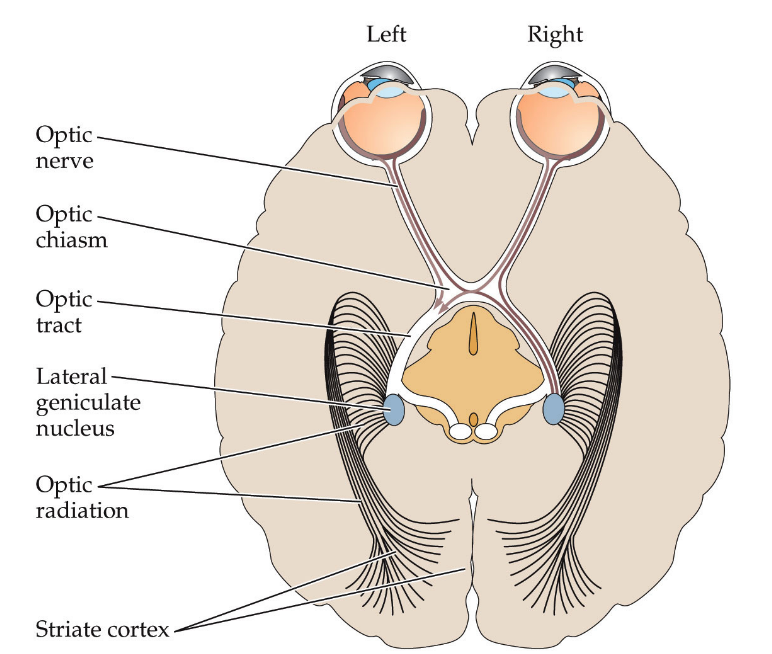
\includegraphics[width=45mm]{figs/l3/cortical_pathways2.png}
\end{column}

 \begin{column}{50mm}
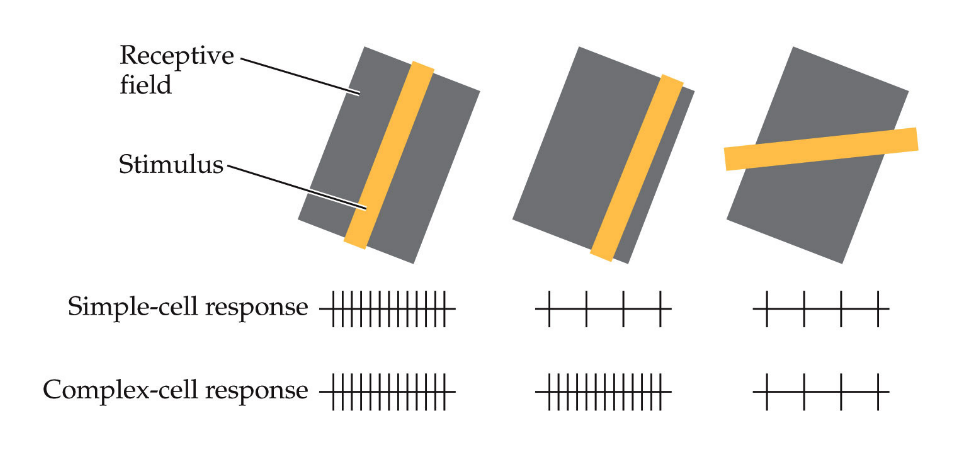
\includegraphics[width=50mm]{figs/l3/complex_cell_response.png}
 \end{column}
\end{columns}
\end{overlayarea}
\end{frame}




\begin{frame}
\frametitle{Edge detection}
\begin{overlayarea}{110mm}{60mm}
  \begin{center}
\includegraphics<1>[width=70mm]{figs/l5/houses_edges.png}
 \end{center}
\end{overlayarea}
\begin{itemize}
 \item cells in primary visual cortex have small receptive fields and respond to edges of varying orientations
 \item How do you know which edges go together and which ones don't?
\end{itemize}
\end{frame}


\begin{frame}
\frametitle{Mid-level vision}
\begin{itemize}
\setlength{\itemsep}{5pt}
 \item A loosely defined stage of visual processing that comes after basic features have been extracted from the image and before object recognition and scene understanding
 \item Involves the perception of edges and surfaces
 \item Determines which regions of an image should be grouped together into objects
\end{itemize}
\end{frame}


\begin{frame}
\frametitle{Finding edges: computers are not as good as humans}
\only<1>{
\begin{itemize}
 \item Sometimes computers don't find enough edges
\end{itemize}
}
\only<2>{
\begin{itemize}
 \item<2>Sometimes computers find too many edges 
\end{itemize}
}
  \begin{center}
\includegraphics<1>[width=100mm]{figs/l5/under_segmentation.png}
\includegraphics<2>[width=100mm]{figs/l5/over_segmentation.png}
 \end{center}
\end{frame}

\begin{frame}
\frametitle{Human contour perception is inferential}
   \begin{center}
\includegraphics<1>[width=50mm]{figs/l5/house_kanizsa.png}

\vspace{5mm}
Kanizsa's illusory contours
 \end{center}

\end{frame}


\begin{frame}
\begin{overlayarea}{120mm}{40mm}
\begin{center}
\includegraphics<1>[width=60mm]{../../../figures/bregman_Bs.png}
\includegraphics<2>[width=20mm]{../../../figures/banana_penetrates_brick.png}
\includegraphics<3->[width=60mm]{../../../figures/amodal_michotte.png}
\end{center}
\only<4>{
What kind of regularities in the stimulus are taken as evidence for a contour in the world?}
\end{overlayarea}
\end{frame}



\begin{frame}
\frametitle{Gestalt grouping rules}
\begin{overlayarea}{110mm}{70mm}
\begin{columns}[T]
\begin{column}{50mm}
\begin{center}
 \begin{itemize}
\setlength{\itemsep}{50pt}
 \item Good continuation
 \item<2-> Similarity
 \item<3-> Proximity
\end{itemize}
\end{center}
\end{column}

 \begin{column}{50mm}
\begin{center}
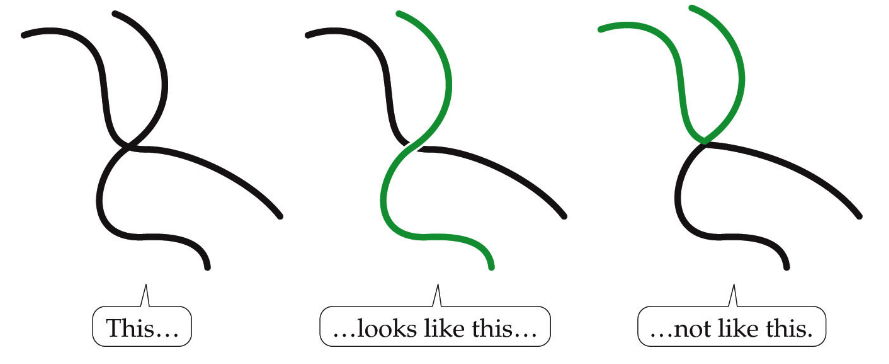
\includegraphics[width=45mm]{figs/l5/good_continuation.png}

\vspace{3mm}
\includegraphics<2->[width=15mm]{figs/l5/gestalt_similarity.png}

\vspace{8mm}
\includegraphics<3->[width=15mm]{figs/l5/gestalt_proximity.png}
\end{center}
 \end{column}
\end{columns}
\end{overlayarea}
\end{frame}


\begin{frame}
\frametitle{Gestalt grouping rules}
\begin{overlayarea}{110mm}{70mm}
\begin{columns}[T]
\begin{column}{50mm}
\begin{center}
 \begin{itemize}
\setlength{\itemsep}{50pt}
 \item Good continuation
\end{itemize}
\end{center}
\end{column}

 \begin{column}{50mm}
\begin{center}
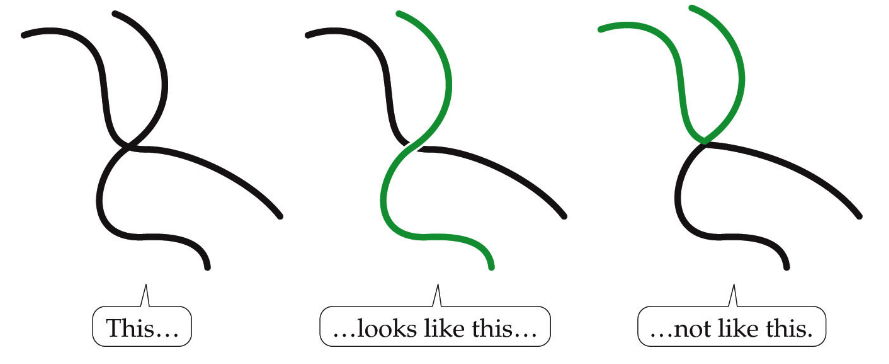
\includegraphics[width=45mm]{figs/l5/good_continuation.png}
\end{center}
 \end{column}
\end{columns}
\begin{center}
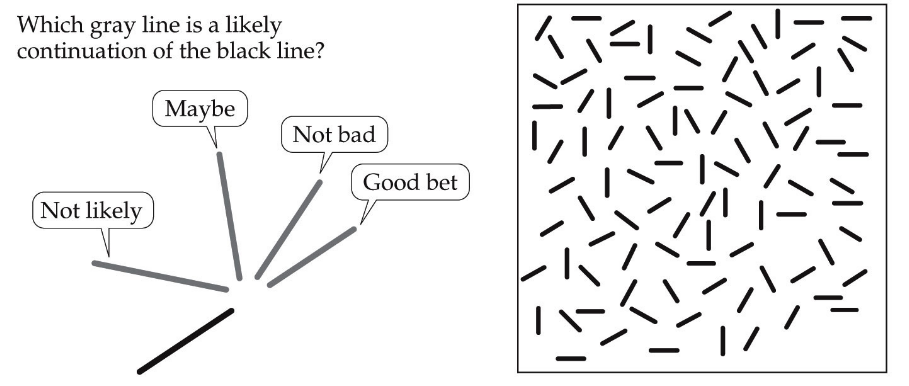
\includegraphics[width=70mm]{figs/l5/contour_completion_field.png}
\end{center}

\end{overlayarea}
\end{frame}



\begin{frame}
\frametitle{Gestalt grouping rules}
\begin{overlayarea}{110mm}{80mm}
\begin{columns}[T]
\begin{column}{70mm}
\begin{center}
 \begin{itemize}
\setlength{\itemsep}{50pt}
 \item Proximity and similarity serve texture segmentation
\end{itemize}
\end{center}
\end{column}

 \begin{column}{30mm}
\begin{center}
\vspace{3mm}
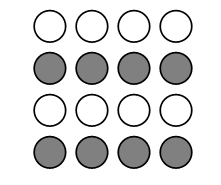
\includegraphics[width=15mm]{figs/l5/gestalt_similarity.png}
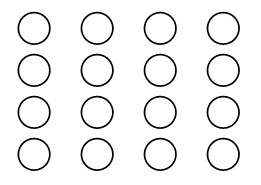
\includegraphics[width=15mm]{figs/l5/gestalt_proximity.png}
\end{center}
 \end{column}
\end{columns}
\begin{center}

\includegraphics[height=40mm]{figs/l5/texture_segmentation.png}


\includegraphics[width=60mm]{figs/l5/odog_scales.png}
\end{center}
\end{overlayarea}
\end{frame}


\begin{frame}
\begin{block}{Activity}
Explore the Gestalt grouping principles with the activity on the following webpage \url{http://sites.sinauer.com/wolfe4e/wa04.01.html}
\end{block}
\end{frame}


\begin{frame}
 \frametitle{Gestalt rules at work}
\begin{center}
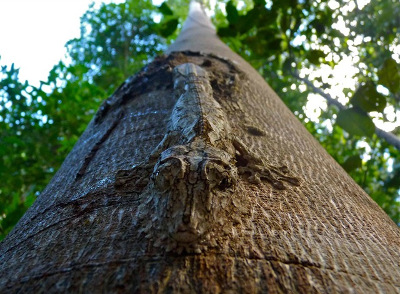
\includegraphics[height=30mm]{figs/l5/camouflage_similarity.jpg}
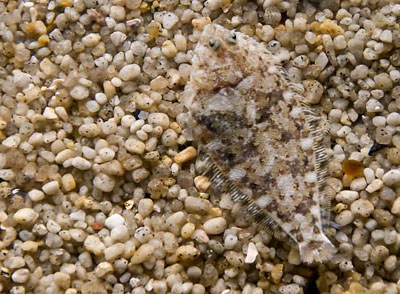
\includegraphics[height=30mm]{figs/l5/camouflage_similarity2.jpg}
\end{center}

\only<2>{\centering\textcolor{blue}{Camouflage}}
\end{frame}



\begin{frame}
 \frametitle{Ambiguous figures}

\begin{center}
\includegraphics<1>[width=70mm]{figs/l5/duck_rabbit.png}
\includegraphics<2>[width=70mm]{figs/l5/necker_cube.png}
\includegraphics<3>[width=80mm]{figs/l5/accidental_viewpoint.png}
\end{center}
\only<3->{
\begin{itemize}
 \item \textbf{accidental viewpoints:} to see the arbitrary shapes just like the four squares would be quite a coincidence
 \item chances for this are so slim that the visual system might refuse this possibility
\end{itemize}
}
\end{frame}

\begin{frame}
 \frametitle{What is figure and what is ground?}
\begin{center}
\includegraphics<1>[width=40mm]{figs/l5/figure_ground.png}
\end{center}

\end{frame}



\begin{frame}
 \frametitle{What is figure and what is ground?}

\begin{itemize}
 \item figure-ground assignment is a critical step on the path from image to object recognition
 \item happens as early as in the first extrastriate cortical area V2
 \item neurons are sensitive to border-ownership
\end{itemize}

\begin{center}
\includegraphics<1>[width=40mm]{figs/l5/figure_side_selectivity.png}
\end{center}
\end{frame}


\begin{frame}
 \frametitle{Principles of figure-ground assignment}
\begin{columns}[T]
 \begin{column}{50mm}
\begin{itemize}[<+->]
\setlength{\itemsep}{10pt}
 \item surroundedness
 \item size
 \item symmmetry
 \item parallelism
 \item extremal edges
 \item relative motion
\end{itemize}
 \end{column}

 \begin{column}{60mm}
\begin{center}
\includegraphics<1-3>[width=40mm]{figs/l5/figure_ground.png}
\includegraphics<4>[width=40mm]{figs/l5/parallel_figure.png}
\includegraphics<5>[width=40mm]{figs/l5/extremal_edges.png}
\includegraphics<7>[width=40mm]{figs/l5/rubin_vase.png}
\end{center}
 \end{column}
\end{columns}
\end{frame}

\begin{frame}
 \frametitle{Principles of figure-ground assignment}
\begin{center}
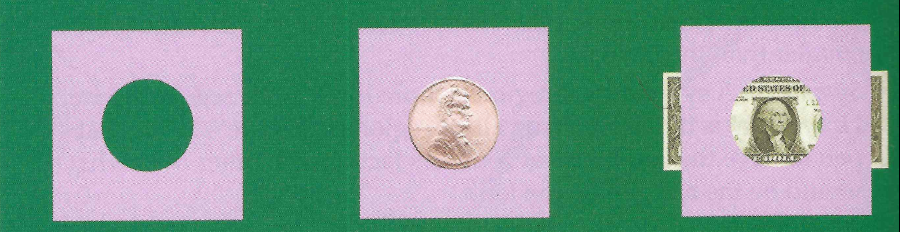
\includegraphics[width=100mm]{figs/l5/figures_holes.png}
\begin{itemize}
 \item size, surroundedness, symmetry, parallelism 
 \item[$\rightarrow$] purple squares = figures
 \item[]
 \item What about the circle in the middle of each square?
 \item<2-> only the one in the middle is seen as separate object, the other two are seen as wholes, why?
\end{itemize}
\end{center}
\end{frame}

\begin{frame}
 \frametitle{Dealing with occlusion in 2D: Relatability}
\begin{overlayarea}{110mm}{90mm}
\begin{center}
\includegraphics<1-2>[width=50mm]{figs/l5/relatability.png}
\only<3->{\vspace{8mm}}
\includegraphics<3>[width=70mm]{../../../figures/amodal_michotte.png}
\end{center}
\only<2->{
\begin{itemize}
 \item complete line fragments that can be related by simple curves
 \item visual system ``unwilling'' to propose complex relationships between line fragments
 \item<3-> complete smooth curves = \textcolor{blue}{heuristic} 
\end{itemize}
}
\end{overlayarea}
\end{frame}


\begin{frame}
 \frametitle{Dealing with occlusion in 3D: T-junctions}
\begin{overlayarea}{110mm}{50mm}
\begin{center}
\includegraphics<1>[width=70mm]{figs/l5/T_junctions.png}
\end{center}
\end{overlayarea}
\end{frame}

\begin{frame}
 \frametitle{T-junctions and (non-)accidental viewpoints}
\begin{overlayarea}{110mm}{50mm}
\begin{center}
\includegraphics<1>[width=90mm]{figs/l5/accidental_viewpoints_frank.png}
\includegraphics<2>[width=90mm]{figs/l5/canonical_viewpoints.png}
\end{center}
\end{overlayarea}
\end{frame}



\begin{frame}
 \frametitle{Summary}
\begin{itemize}
\setlength{\itemsep}{5pt}
 \item after early vision extracts basic features from the visual input, mid-level vision organizes these features into the regions, surfaces and objects that provide the basis for object recognition
 \item visual system applies rules for image segmentation, edge finding processes that divide regions from each other
 \item visual system applies rules for grouping such as similarity, symmetry, parallelism, proximity ...
 \item together these principles allow figure ground assignment
 \item visual systems avoids accidents
\end{itemize}

\end{frame}




\begin{frame}
 \frametitle{References}
\begin{small}
\begin{itemize}
 \item  Wolfe, J.M., Kluender, K.R. \& Levi, D.M. (2012).\textit{Sensation \& Perception}. Sinauer Associates: Sunderland, MA. 
\end{itemize}
\end{small}
\end{frame}


\end{document}